\documentclass[titlepage, dvipsnames]{article}

\usepackage[%
left=2.5cm,%
right=2.5cm,%
top=2cm,%
bottom=2cm,%
]{geometry}%
\usepackage{tikz}
\usetikzlibrary{shapes,snakes}
\usepackage{amsmath,amssymb,amsthm}
\usepackage{graphicx}
\usepackage{subcaption}
\usepackage{float}
\usepackage{enumitem}
\usepackage{etoc}
\usepackage[framemethod=tikz]{mdframed}
\usepackage[answerdelayed]{exercise}
\usepackage{subfiles}
\usepackage{wrapfig}
\usepackage{multicol}

\graphicspath{ {./images/} }

% custom commands
\let\bold\bfseries
\newcommand{\N}{\mathbb{N}}
\newenvironment{TODO}[1]
    {\textcolor{red}{\textbf{TODO}}
     #1
     \\
    }


\usepackage[utf8]{inputenc}
\usepackage[german]{babel}

% Theoreme etc.
\theoremstyle{plain}
\newmdtheoremenv[
  backgroundcolor=red!10,
  hidealllines=true,
  innerleftmargin=10pt,
  innerrightmargin=10pt,
  innertopmargin=0pt,
]{theorem}{Theorem}[section]
\newtheorem{corollary}{Corollary}[theorem]
\newtheorem{lemma}[theorem]{Lemma}
\theoremstyle{remark}
\newtheorem*{remark}{Remark}
\newmdtheoremenv[
    topline = true,
    bottomline = true,
    leftline = false,
    rightline = false,
    innertopmargin = 10pt,
    innerbottommargin = 10pt,
]{example}{example}[section]
\theoremstyle{definition}
\newmdtheoremenv[
  backgroundcolor=brown!20,
  hidealllines=true,
  innerleftmargin=10pt,
  innerrightmargin=10pt,
  innertopmargin=0pt,
]{definition}{Definition}[subsection]


\title{Parallel Programming PVW FS19}
\author{Lasse Meinen}

\begin{document}
    \renewcommand{\figurename}{Fig.}
    \renewcommand{\contentsname}{Table of Contents}
    \renewcommand{\thesubfigure}{\roman{subfigure}}
    
    \renewcommand{\ExerciseHeaderTitle}{\ExerciseTitle}
    \renewcommand{\ExerciseHeader}{\centerline{\textbf{\large\ExerciseName\ExerciseHeaderNB\ExerciseHeaderTitle\ExerciseHeaderOrigin}}\\}
    \renewcommand{\ExerciseListHeader}{\ExerciseHeaderDifficulty%
    \textbf{\ExerciseHeaderNB .%
    \ \ExerciseHeaderTitle \newline}%
    \ExerciseHeaderOrigin\ignorespaces}
    \renewcommand{\AnswerListHeader}{\textbf{\ExerciseHeaderNB. \ \ExerciseHeaderTitle}}
    \setlength{\Exesep}{1\baselineskip}    
    \setlength{\QuestionBefore}{.2em}
    \setlength{\QuestionIndent}{2em}
    
    \makeatletter 
    \begin{titlepage}
        \begin{center}
            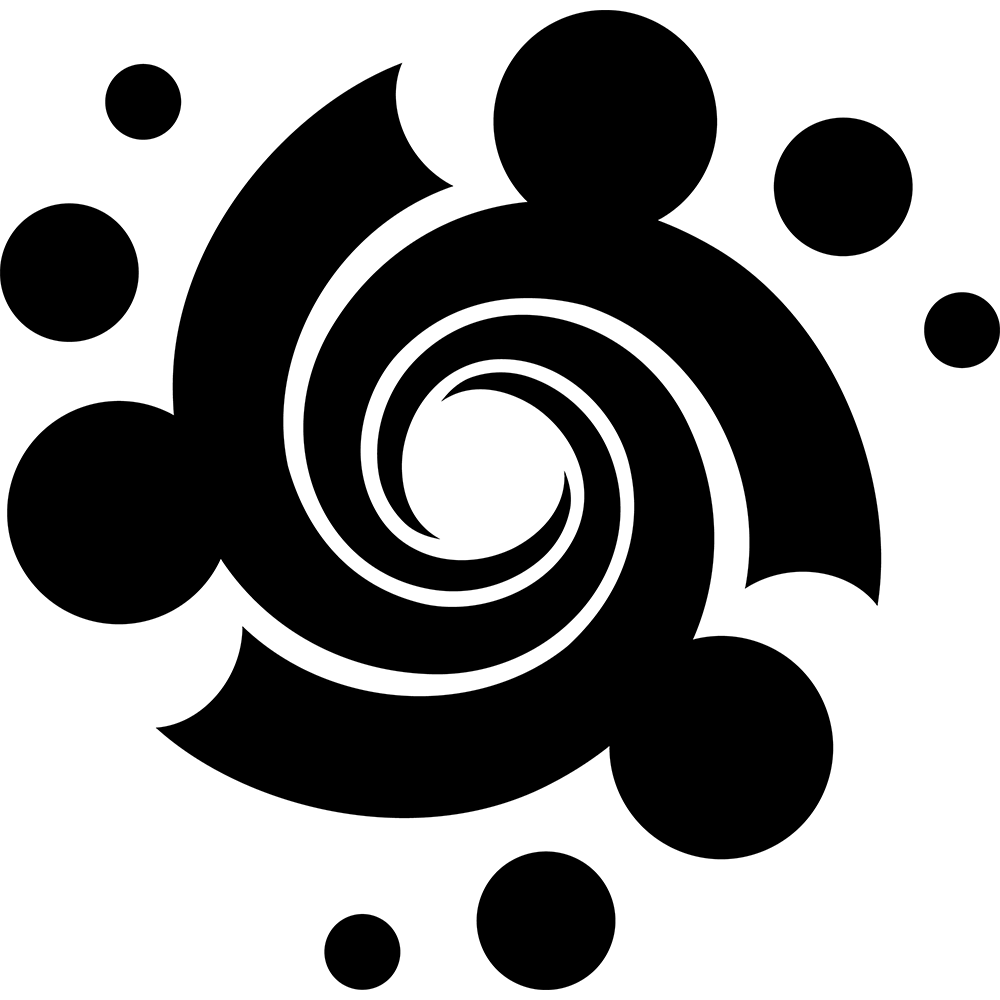
\includegraphics[width=0.7\linewidth]{spirale_black1000x1000.png}\\[4ex]
            \huge \textbf{\@title} \\[2ex] 
            \Large \textbf{Last updated on 15.06.2019} \\[2ex]
            \large written by \@author\\[2ex] 
            \large pprog-pvw-skript@vis.ethz.ch \\[50ex]
        \end{center}
    \end{titlepage}
    \makeatother
    \thispagestyle{empty}
    \newpage

    \subfile{Disclaimer}
    \newpage
    
    \setcounter{page}{1} %Start the actually document on page 1
    
    \tableofcontents
    \newpage
    \subfile{1.Introduction}
    \newpage
    \subfile{2.Parallelism}
    \newpage
    \subfile{3.Concurrency}
    \newpage
    \subfile{4.AdditionalTopics}
    \newpage
\end{document}